\documentclass[12pt, a4paper]{report}

% Packages
\usepackage[utf8]{inputenc}
\usepackage{graphicx}
\usepackage{geometry}
\usepackage{setspace}
\usepackage{titlesec}
\usepackage{hyperref}
\usepackage{listings}
\usepackage{xcolor}
\usepackage{float}
\usepackage{caption}
\usepackage{subcaption}
\usepackage{fancyhdr}
\usepackage{mathptmx} % Times New Roman font

% Page Layout (Top=1, Bottom=1, Right=1, Left=1.25)
\geometry{
    left=1.25in,
    right=1in,
    top=1in,
    bottom=1in
}

% Line Spacing (1.5)
\onehalfspacing

% Paragraph Style (Justified)
\setlength{\parindent}{0pt}
\setlength{\parskip}{1em}

% Hyperlink Setup
\hypersetup{
    colorlinks=true,
    linkcolor=black,
    filecolor=black,      
    urlcolor=black,
    citecolor=black,
    pdftitle={Personal Finance Manager Report},
    pdfpagemode=FullScreen,
}

% Code Listing Style
\definecolor{codegreen}{rgb}{0,0.6,0}
\definecolor{codegray}{rgb}{0.5,0.5,0.5}
\definecolor{codepurple}{rgb}{0.58,0,0.82}
\definecolor{backcolour}{rgb}{0.95,0.95,0.92}

\lstdefinestyle{mystyle}{
    backgroundcolor=\color{backcolour},   
    commentstyle=\color{codegreen},
    keywordstyle=\color{magenta},
    numberstyle=\tiny\color{codegray},
    stringstyle=\color{codepurple},
    basicstyle=\ttfamily\footnotesize,
    breakatwhitespace=false,         
    breaklines=true,                 
    captionpos=b,                    
    keepspaces=true,                 
    numbers=left,                    
    numbersep=5pt,                  
    showspaces=false,                
    showstringspaces=false,
    showtabs=false,                  
    tabsize=2
}

\lstset{style=mystyle}

% Heading Formatting
% Chapter Title: 16pt, Bold, Centered
\titleformat{\chapter}[display]
{\normalfont\fontsize{16}{19.2}\selectfont\bfseries\centering}{\chaptertitlename\ \thechapter}{20pt}{\fontsize{16}{19.2}\selectfont}

% Section Heading: 14pt, Bold
\titleformat{\section}
{\normalfont\fontsize{14}{16.8}\selectfont\bfseries}{\thesection}{1em}{}

% Subsection Heading: 12pt, Bold
\titleformat{\subsection}
{\normalfont\fontsize{12}{14.4}\selectfont\bfseries}{\thesubsection}{1em}{}

% Caption Formatting: Bold, 12pt
\captionsetup{font={bf, small}, labelfont=bf}

\begin{document}

% -------------------------------------------------------------------
% Title Page
% -------------------------------------------------------------------
\begin{titlepage}
    \begin{center}
        \vspace*{1cm}
        
        \textbf{\large PERSONAL FINANCE MANAGER (PFM)}
        
        \vspace{1.5cm}
        
        \textbf{A PROJECT REPORT}
        
        \vspace{1.5cm}
        
        \textbf{SUBMITTED BY}
        
        \textbf{[Student Name]} \\
        \textbf{TU Registration No.: [Reg. No.]} \\
        \textbf{Campus Roll No.: [Roll No.]}
        
        \vspace{1.5cm}
        
        \textbf{SUBMITTED TO}
        
        \textbf{Department of Computer Science and Information Technology} \\
        \textbf{[Campus/College Name]} \\
        \textbf{Tribhuvan University}
        
        \vspace{1.5cm}
        
        In partial fulfillment of the requirements for the degree of \\
        \textbf{Bachelor of Science in Computer Science and Information Technology (B.Sc. CSIT)}
        
        \vspace{1.5cm}
        
        \textbf{[Month, Year]}
        
    \end{center}
\end{titlepage}

% -------------------------------------------------------------------
% Preliminary Pages
% -------------------------------------------------------------------
\pagenumbering{roman} % Roman numerals for prelim pages
\setcounter{page}{2} % Start counting from certificate (Title page is technically i)

% Supervisor's Recommendation
\newpage
\begin{center}
    \textbf{\large TRIBHUVAN UNIVERSITY} \\
    \textbf{\large INSTITUTE OF SCIENCE AND TECHNOLOGY} \\
    \textbf{\large [CAMPUS/COLLEGE NAME]} \\
    \textbf{\large DEPARTMENT OF COMPUTER SCIENCE AND INFORMATION TECHNOLOGY}
    
    \vspace{1cm}
    
    \textbf{\large SUPERVISOR'S RECOMMENDATION}
\end{center}
\vspace{0.5cm}
I hereby recommend that this project report prepared by \textbf{[Student Name]} entitled ``\textbf{Personal Finance Manager (PFM)}'' be accepted as a partial fulfillment of the requirements for the degree of B.Sc. in Computer Science and Information Technology. In my best knowledge, this is an original work in computer science.

\vspace{2cm}

\noindent ................................................ \\
\textbf{[Supervisor Name]} \\
Supervisor \\
Department of Computer Science and Information Technology \\
[Campus Name] \\
[Date]

% Letter of Approval
\newpage
\begin{center}
    \textbf{\large TRIBHUVAN UNIVERSITY} \\
    \textbf{\large INSTITUTE OF SCIENCE AND TECHNOLOGY} \\
    \textbf{\large [CAMPUS/COLLEGE NAME]} \\
    \textbf{\large DEPARTMENT OF COMPUTER SCIENCE AND INFORMATION TECHNOLOGY}
    
    \vspace{1cm}
    
    \textbf{\large LETTER OF APPROVAL}
\end{center}
\vspace{0.5cm}
We certify that we have examined this project report entitled ``\textbf{Personal Finance Manager (PFM)}'' submitted by \textbf{[Student Name]} and reviewed the candidate's project work. We recommend that the project report be accepted as a partial fulfillment of the requirements for the degree of B.Sc. in Computer Science and Information Technology.

\vspace{1.5cm}

\noindent \textbf{Evaluation Committee}

\vspace{1cm}

\noindent 
\begin{tabular}{lr}
................................................ & ................................................ \\
\textbf{[Supervisor Name]} & \textbf{[Head of Department Name]} \\
Supervisor & Head of Department \\
\end{tabular}

\vspace{1.5cm}

\noindent ................................................ \\
\textbf{[External Examiner Name]} \\
External Examiner

\vspace{0.5cm}

\noindent Date: ................................................


% Acknowledgement
\newpage
\chapter*{ACKNOWLEDGEMENT}
\addcontentsline{toc}{chapter}{Acknowledgement}

I would like to express my sincere gratitude to my supervisor, \textbf{[Supervisor Name]}, for their invaluable guidance, encouragement, and support throughout the course of this project. Their insights and feedback were instrumental in shaping the direction of this work.

I am also grateful to \textbf{[Head of Department Name]}, Head of the Department of Computer Science and Information Technology, for providing the necessary facilities and resources.

I would like to thank my friends and family for their unwavering support and motivation during the development of this project.

\vspace{1cm}

\noindent \textbf{[Student Name]} \\
[Date]


% Abstract
\newpage
\chapter*{ABSTRACT}
\addcontentsline{toc}{chapter}{Abstract}

Managing personal finances is a crucial aspect of modern life, yet many individuals struggle with tracking expenses due to the tedious nature of manual entry and categorization. The \textbf{Personal Finance Manager (PFM)} is a hybrid mobile and web application designed to simplify expense tracking through the power of Natural Language Processing (NLP) and Artificial Intelligence.

The system allows users to log expenses using natural language phrases (e.g., ``spent 500 on lunch''), which are then parsed and categorized automatically by Google's Gemini AI. Built using a robust tech stack comprising \textbf{React.js} for the frontend, \textbf{FastAPI (Python)} for the backend, \textbf{Supabase (PostgreSQL)} for the database, and \textbf{Capacitor} for mobile deployment, the application offers a seamless cross-platform experience. Key features include intelligent expense categorization, multi-group management for shared expenses, real-time financial analytics, and a voice-enabled interface. This project demonstrates the effective integration of modern web technologies and Generative AI to solve real-world financial management problems.

\vspace{0.5cm}
\noindent \textbf{Keywords:} \textit{Personal Finance, Expense Tracking, Natural Language Processing, Artificial Intelligence, React, FastAPI, Gemini API.}

% Table of Contents
\newpage
\tableofcontents

% List of Figures
\newpage
\listoffigures

% List of Tables
\newpage
\listoftables

% List of Abbreviations
\newpage
\chapter*{LIST OF ABBREVIATIONS}
\addcontentsline{toc}{chapter}{List of Abbreviations}
\begin{tabbing}
    \hspace{3cm} \= \kill
    PFM \> Personal Finance Manager \\
    NLP \> Natural Language Processing \\
    AI \> Artificial Intelligence \\
    API \> Application Programming Interface \\
    SDLC \> Software Development Life Cycle \\
    UML \> Unified Modeling Language \\
    DFD \> Data Flow Diagram \\
    ER \> Entity Relationship \\
    UI/UX \> User Interface / User Experience
\end{tabbing}

% -------------------------------------------------------------------
% Main Content
% -------------------------------------------------------------------
\newpage
\pagenumbering{arabic} % Arabic numerals for main chapters
% Reset to 1 for introduction
\setcounter{page}{1}

\chapter{INTRODUCTION}

\section{Introduction}
In an era of digital payments and complex financial obligations, effective management of personal finances has become a necessity. Individuals often struggle to keep track of their daily expenses, leading to poor financial health and lack of savings. Traditional methods of expense tracking, such as manual ledgers or spreadsheets, are time-consuming and prone to human error. Even mobile applications often require tedious manual entry of date, amount, category, and description for every transaction, leading to user drop-off.

The \textbf{Personal Finance Manager (PFM)} is designed to address these challenges by leveraging the power of Artificial Intelligence (AI) and Natural Language Processing (NLP). By allowing users to input expenses in natural language---as if they were texting a friend---the system removes the friction of manual data entry. Integrated with Google's Gemini API, the system intelligently understands the context of the expense, categorizes it automatically, and stores it for analysis. This project aims to democratize financial literacy and ease of management through a modern, user-friendly interface accessible on both web and mobile platforms.

\section{Problem Statement}
Despite the availability of numerous financial management tools, several key issues persist:

\begin{enumerate}
    \item \textbf{High Data Entry Friction:} Users find it cumbersome to manually select categories, dates, and payment modes for every small transaction.
    \item \textbf{Lack of Intelligent Categorization:} Most apps rely on rigid, pre-defined rules that fail to understand context (e.g., ``coffee with client'' might be a business expense, not just ``Food'').
    \item \textbf{Complex Interfaces:} Many financial apps are cluttered with complex charts and features that overwhelm the average user.
    \item \textbf{Fragmented Experience:} Users often need separate apps for personal tracking and shared expenses (e.g., splitting bills with roommates).
\end{enumerate}

\section{Objectives}
The primary objective of this project is to develop a smart, NLP-powered personal finance management system. The specific objectives are:

\begin{enumerate}
    \item \textbf{To implement Natural Language Expense Logging:} Enable users to log expenses using simple text commands (e.g., ``200 for taxi'').
    \item \textbf{To automate Expense Categorization:} Utilize Generative AI (Google Gemini) to accurately categorize transactions based on description and context.
    \item \textbf{To provide Real-time Analytics:} Develop interactive dashboards to visualize spending habits, trends, and budget adherence.
    \item \textbf{To support Multi-Group Management:} Facilitate shared expense tracking for families, roommates, or trip groups.
    \item \textbf{To ensure Cross-Platform Accessibility:} Deploy the application as a Progressive Web App (PWA) and an Android application.
\end{enumerate}

\section{Scope and Limitation}

\subsection{Scope}
The scope of the PFM project covers:
\begin{itemize}
    \item \textbf{User Management:} Secure authentication and profile management via Supabase.
    \item \textbf{Expense Tracking:} Functionality to add, edit, and delete expenses using both text-based NLP input and manual forms.
    \item \textbf{AI Integration:} Integration with Google Gemini API for parsing unstructured text into structured JSON data.
    \item \textbf{Visualization:} Graphical representation of financial data using charts and graphs.
    \item \textbf{Platform:} The application is scoped for Web browsers (Chrome, Firefox, Safari) and Android devices (via Capacitor).
\end{itemize}

\subsection{Limitation}
\begin{itemize}
    \item \textbf{Internet Dependency:} The AI features require an active internet connection to communicate with the Gemini API.
    \item \textbf{Language Support:} Currently, the NLP parser is optimized for English and Hinglish (Hindi-English mix) and may not support other regional languages effectively.
    \item \textbf{Bank Integration:} The system does not currently support automatic SMS reading or direct bank account syncing due to security and privacy constraints.
    \item \textbf{Scalability Constraints:} The free tier of Supabase and Gemini API imposes rate limits which may affect scalability under high load.
\end{itemize}

\section{Development Methodology}
The project follows the \textbf{Agile Software Development Methodology}. Agile was chosen for its iterative nature, allowing for continuous feedback and improvement. 
The development was divided into 2-week sprints:
\begin{itemize}
    \item \textbf{Sprint 1:} Requirement gathering and UI protoyping.
    \item \textbf{Sprint 2:} Backend API development and Database setup.
    \item \textbf{Sprint 3:} Frontend integration and AI implementation.
    \item \textbf{Sprint 4:} Testing, Bug fixes, and Documentation.
\end{itemize}

\section{Report Organization}
This project report is organized into five chapters:
\begin{itemize}
    \item \textbf{Chapter 1: Introduction} outlines the project background, problem, objectives, and scope.
    \item \textbf{Chapter 2: Background Study and Literature Review} discusses fundamental concepts and reviews similar existing systems.
    \item \textbf{Chapter 3: System Analysis and Design} details the requirement analysis, feasibility, and comprehensive system design using UML diagrams.
    \item \textbf{Chapter 4: Implementation and Testing} describes the tools used, implementation details, and testing strategies.
    \item \textbf{Chapter 5: Conclusion and Future Recommendations} summarizes the project outcomes and suggests future improvements.
\end{itemize}

\chapter{BACKGROUND STUDY AND LITERATURE REVIEW}

\section{Background Study}
\textit{(Description of fundamental theories, general concepts and terminologies related to the project)}

To understand the development of the Personal Finance Manager, it is essential to grasp the fundamental concepts and technologies involved:

\begin{itemize}
    \item \textbf{Personal Finance Management (PFM):} The practice of budgeting, saving, and spending monetary resources over time, taking into account various financial risks and future life events.
    \item \textbf{Natural Language Processing (NLP):} A subfield of artificial intelligence describing the interaction between computers and human language. In this project, NLP is used to interpret unstructured expense descriptions (e.g., "taxi 500") into structured data (Category: Travel, Amount: 500).
    \item \textbf{Large Language Models (LLMs):} Deep learning algorithms that can recognize, summarize, translate, predict, and generate text and other forms of content based on knowledge gained from massive datasets. We utilize Google's Gemini model for this purpose.
    \item \textbf{Client-Server Architecture:} A distributed application structure that partitions tasks or workloads between the providers of a resource or service, called servers, and service requesters, called clients. PFM uses React as the client and FastAPI as the server.
    \item \textbf{REST API (Representational State Transfer):} An architectural style for an application program interface (API) that uses HTTP requests to access and use data.
\end{itemize}

\section{Literature Review}
\textit{(Review of the similar projects, theories done by other researchers)}

Several personal finance management applications exist in the market, each offering various features for expense tracking and budgeting. A critical review of these systems provides insights into current standards and gaps.

\subsection{Mint (Intuit)}
Mint was one of the most popular PFM tools, offering automatic bank synchronization, budgeting, and credit score tracking.
\begin{itemize}
    \item \textbf{Overview:} Aggregates all financial accounts in one place.
    \item \textbf{Theory:} Automates tracking through direct bank connections.
    \item \textbf{Limitations:} Recently discontinued/migrated to Credit Karma, heavily ad-supported, privacy concerns with bank data.
\end{itemize}

\subsection{You Need A Budget (YNAB)}
YNAB focuses on zero-based budgeting, encouraging users to give every dollar a job.
\begin{itemize}
    \item \textbf{Theory:} Proactive budgeting rather than reactive tracking.
    \item \textbf{Limitations:} Expensive subscription model, steep learning curve for new users, requires manual discipline.
\end{itemize}

\subsection{Splitwise}
Specifically designed for splitting bills and shared expenses.
\begin{itemize}
    \item \textbf{Theory:} Simplified group debt simplification algorithms.
    \item \textbf{Limitations:} Not a full PFM (lacks personal budgeting, net worth tracking), limited analytics for individual spending.
\end{itemize}

\subsection{Research Gap}
Most existing research and products focus either on fully automated bank syncing (which raises privacy/security issues for local contexts) or fully manual entry (which causes user fatigue). There is a lack of "Hybrid" systems that facilitate manual entry through intelligent automation like NLP commands. This project aims to fill this gap.

\chapter{SYSTEM ANALYSIS AND DESIGN}

\section{System Analysis}
System analysis is a process of collecting and interpreting facts, identifying the problems, and decomposition of a system into its components.

\subsection{Requirement Analysis}
Requirement analysis focuses on the tasks that determine the needs or conditions to meet the new or altered product or project, taking account of the possibly conflicting requirements of the various stakeholders.

\subsubsection{Functional Requirements}
Functional requirements define the specific behavior or functions of the system.
\begin{enumerate}
    \item \textbf{Authentication:} Users must be able to register and login securely.
    \item \textbf{Expense Management:} Users can add, edit, and delete expenses using NLP text or manual forms.
    \item \textbf{Categorization:} The system automatically categorizes expenses using AI.
    \item \textbf{Visualization:} Users can view charts and graphs of their spending.
    \item \textbf{Group Expenses:} Users can create groups and split bills.
\end{enumerate}

\begin{figure}[H]
    \centering
    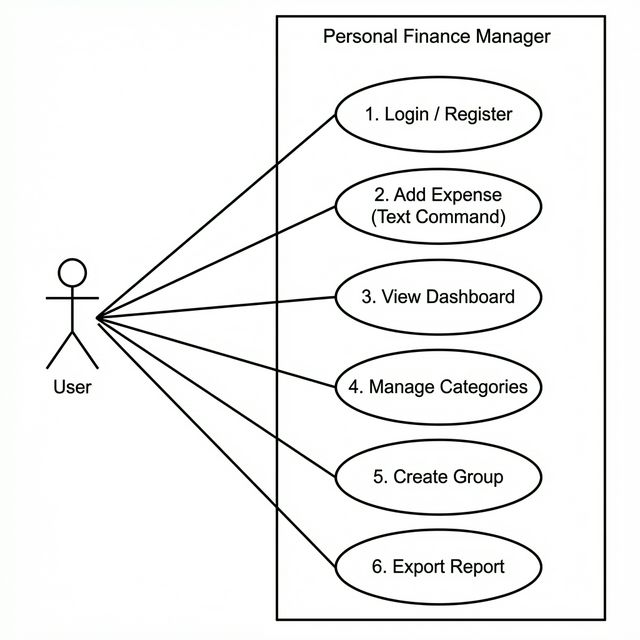
\includegraphics[width=0.8\textwidth]{images/use_case_diagram.png}
    \caption{Use Case Diagram}
    \label{fig:usecase}
\end{figure}

\subsubsection{Non-functional Requirements}
\begin{enumerate}
    \item \textbf{Performance:} Response time for NLP parsing should be under 2 seconds.
    \item \textbf{Reliability:} The system should be available 99.9\% of the time.
    \item \textbf{Security:} Passwords must be hashed; API communication must be over HTTPS.
    \item \textbf{Scalability:} System should handle concurrent users without degradation.
\end{enumerate}

\subsection{Feasibility Analysis}
\subsubsection{Technical Feasibility}
The project uses React (Frontend), Python FastAPI (Backend), and PostgreSQL (Database), which are mature technologies. The integration with Gemini API is supported by official libraries. Thus, the project is technically feasible.

\subsubsection{Operational Feasibility}
The interface is designed to be intuitive, resembling a chat application. No special training is required for users, making it operationally feasible.

\subsubsection{Economic Feasibility}
The project relies on open-source technologies and free-tier cloud services (Supabase, Vercel, Google AI Studio). The primary investment is development time, making it economically feasible.

\subsection{Data Modelling: ER Diagram}
Entity-Relationship (ER) diagram shows the relationships of entity sets stored in a database.

\begin{figure}[H]
    \centering
    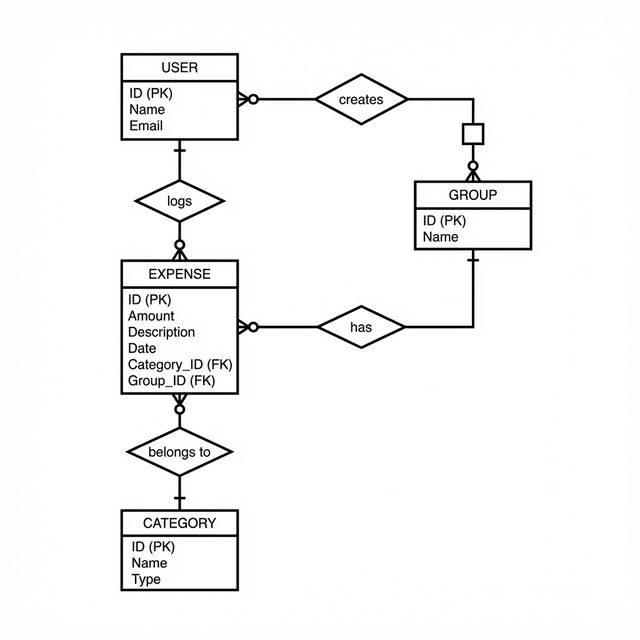
\includegraphics[width=0.9\textwidth]{images/er_diagram.png}
    \caption{Entity Relationship (ER) Diagram}
    \label{fig:er}
\end{figure}

\subsection{Process Modelling: DFD}
Data Flow Diagram (DFD) maps the flow of information for any process or system.

\begin{figure}[H]
    \centering
    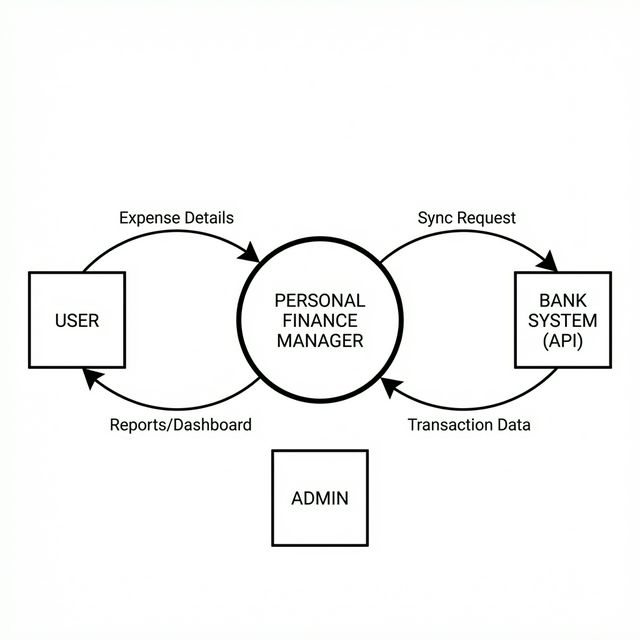
\includegraphics[width=0.9\textwidth]{images/dfd_diagram.png}
    \caption{Data Flow Diagram (Level 0)}
    \label{fig:dfd}
\end{figure}

\subsection{Object Modelling: Object \& Class Diagram}
Class diagram describes the structure of a system by showing the system's classes, their attributes, operations (or methods), and the relationships among objects.

\begin{figure}[H]
    \centering
    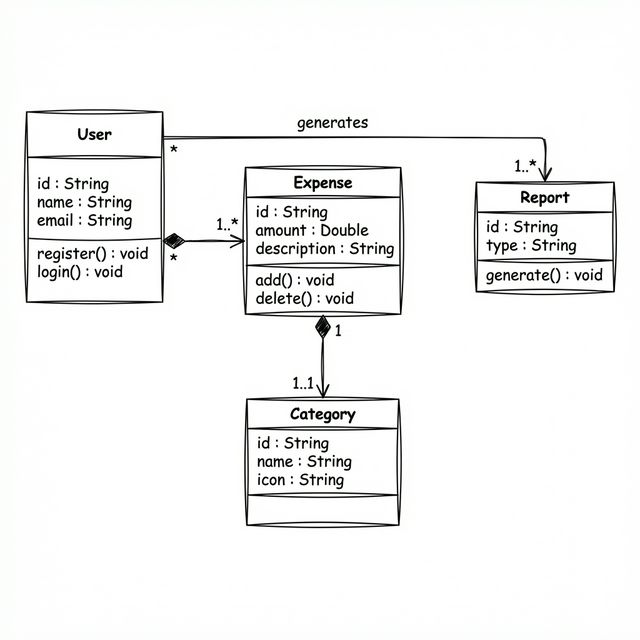
\includegraphics[width=0.9\textwidth]{images/class_diagram.png}
    \caption{Class Diagram}
    \label{fig:class}
\end{figure}

\subsection{Dynamic Modelling: State \& Sequence Diagram}
\subsubsection{State Diagram}
State diagram describes the behavior of a system.

\begin{figure}[H]
    \centering
    \includegraphics[width=0.6\textwidth]{images/state_diagram.png}
    \caption{State Diagram of Expense Processing}
    \label{fig:state}
\end{figure}

\subsubsection{Sequence Diagram}
Sequence diagram shows how objects operate with one another and in what order.

\begin{figure}[H]
    \centering
    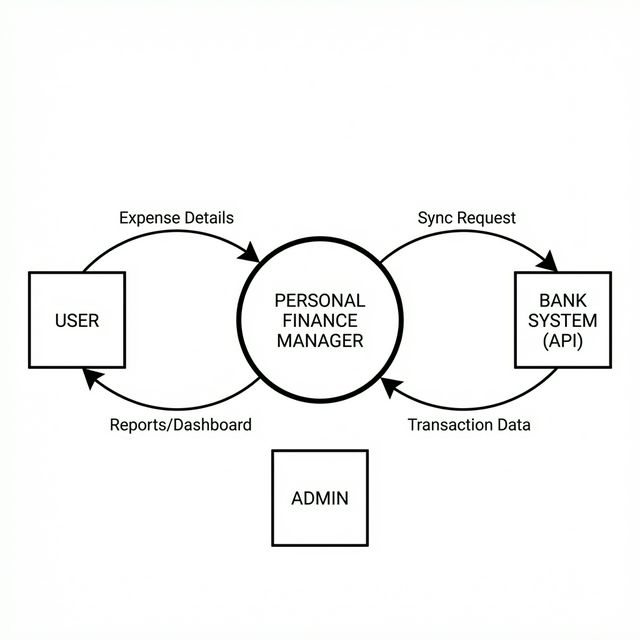
\includegraphics[width=0.9\textwidth]{images/sequence_diagram.png}
    \caption{Sequence Diagram for Adding Expense}
    \label{fig:sequence}
\end{figure}

\subsection{Process Modelling: Activity Diagram}
Activity diagram graphically represents workflows of stepwise activities and actions with support for choice, iteration, and concurrency.

\begin{figure}[H]
    \centering
    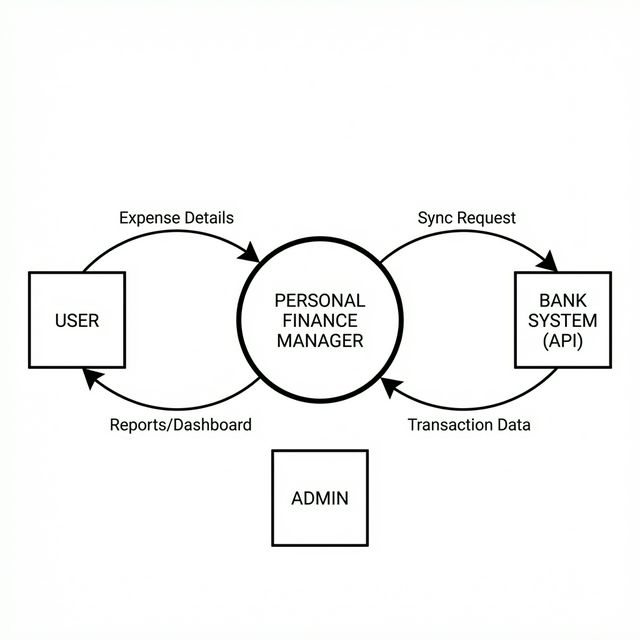
\includegraphics[width=0.6\textwidth]{images/activity_diagram.png}
    \caption{Activity Diagram}
    \label{fig:activity}
\end{figure}

\section{System Design}

\subsection{Architectural Design}
The system uses a \textbf{Client-Server Architecture}. The client is a React Single Page Application (SPA) wrapped in Capacitor for mobile. The server is a REST API built with FastAPI.

\subsection{Database Schema Design}
The database is normalized to 3NF.
\begin{itemize}
    \item \textbf{Users Table:} \texttt{id, restricted\_uid, email, full\_name, created\_at}
    \item \textbf{Categories Table:} \texttt{id, name, type, icon}
    \item \textbf{Expenses Table:} \texttt{id, amount, description, date, user\_id, category\_id, group\_id}
    \item \textbf{Groups Table:} \texttt{id, name, created\_by}
\end{itemize}

\subsection{Interface Design (UI/UX)}
The UI is designed for mobile-first usage. It features a bottom navigation bar, a central floating action button for adding expenses, and a card-based layout for listing transactions.

\subsection{Refinement of Classes and Object}
The initial class model was refined to include helper classes for API communication (\texttt{ApiService}) and state management (\texttt{ExpenseContext}).

\subsection{Component Diagram}
Component diagram depicts how components are wired together to form larger components or software systems.

\begin{figure}[H]
    \centering
    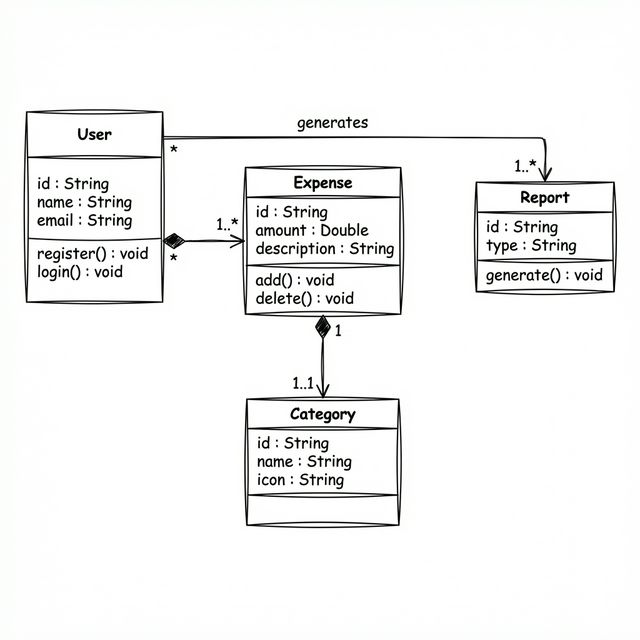
\includegraphics[width=0.7\textwidth]{images/component_diagram.png}
    \caption{Component Diagram}
    \label{fig:component}
\end{figure}

\subsection{Deployment Diagram}
Deployment diagram shows the physical hardware on which the software components run.

\begin{figure}[H]
    \centering
    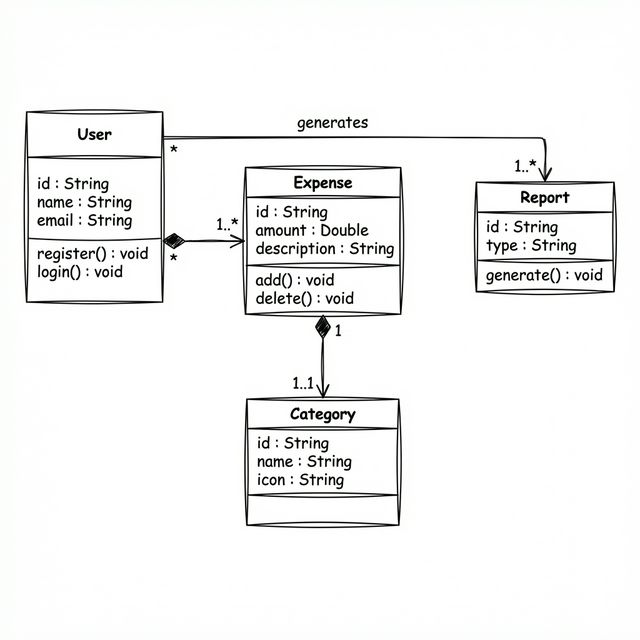
\includegraphics[width=0.7\textwidth]{images/deployment_diagram.png}
    \caption{Deployment Diagram}
    \label{fig:deployment}
\end{figure}

\section{Algorithm Details}
The NLP processing algorithm is central to the system:
\begin{enumerate}
    \item \textbf{Input:} Raw text string $S$ from user.
    \item \textbf{Tokenization:} Send $S$ to LLM with schema instruction.
    \item \textbf{Extraction:} LLM identifies entities: \textit{Amount}, \textit{Currency}, \textit{Category} (mapped to enum), \textit{Date} (relative to absolute).
    \item \textbf{Validation:} Backend defines Pydantic models to validate the JSON structure.
    \item \textbf{Output:} Structured `ExpenseCreate` object or Error.
\end{enumerate}

\chapter{IMPLEMENTATION AND TESTING}

\section{Implementation}

\subsection{Tools Used}
The project was implemented using the following set of tools and technologies:

\begin{itemize}
    \item \textbf{Frontend:} React.js (v18), TailwindCSS (Styling), Recharts (Data Visualization), Capacitor (Mobile Build).
    \item \textbf{Backend:} Python 3.10+, FastAPI (Web Framework), Uvicorn (ASGI Server), Google Gemini SDK (AI).
    \item \textbf{Database Platform:} Supabase (PostgreSQL), Supabase Auth.
    \item \textbf{CASE Tools:} Visual Studio Code, Git, GitHub.
\end{itemize}

\subsection{Implementation Details of Modules}

\subsubsection{User Authentication Module}
Implemented using Supabase Auth. Provides functions for \texttt{signUp()}, \texttt{signInWithPassword()}, and \texttt{signOut()}. Handles session management and JWT token verification.

\subsubsection{Expense Parsing Module (Backend)}
The core feature of the application is the NLP parser. Below is the Python implementation using FastAPI and Gemini:

\begin{lstlisting}[language=Python, caption=Backend API for Expense Parsing]
# backend/api/expenses.py (Snippet)

@router.post("/parse")
async def parse_expense(text: str):
    """
    Parses natural language text into structured expense data.
    """
    prompt = f"""
    Extract the following details from the text: "{text}"
    - Amount (number)
    - Category (Enum: Food, Travel, Bills, Entertainment, Health, Other)
    - Description (string)
    
    Return JSON format only.
    """
    
    response = model.generate_content(prompt)
    try:
        data = json.loads(response.text)
        return {"status": "success", "data": data}
    except json.JSONDecodeError:
        return {"status": "error", "message": "Failed to parse"}
\end{lstlisting}

\subsubsection{Expense Management Module (Frontend)}
The frontend manages state using React Context API to ensure data consistency across components.

\begin{lstlisting}[language=JavaScript, caption=React Context for Expenses]
// src/context/ExpenseContext.js (Snippet)

export const ExpenseProvider = ({ children }) => {
    const [expenses, setExpenses] = useState([]);

    const addExpense = async (text) => {
        const parsed = await api.parseExpense(text);
        if (parsed.status === "success") {
            const newExpense = await api.saveExpense(parsed.data);
            setExpenses([newExpense, ...expenses]);
        }
    };

    return (
        <ExpenseContext.Provider value={{ expenses, addExpense }}>
            {children}
        </ExpenseContext.Provider>
    );
};
\end{lstlisting}

\section{Testing}

\subsection{Test Cases for Unit Testing}
Unit tests were written for individual backend functions, particularly the NLP parsing logic.

\begin{table}[H]
\centering
\begin{tabular}{|l|l|l|l|}
\hline
\textbf{Test ID} & \textbf{Input} & \textbf{Expected Output} & \textbf{Result} \\ \hline
UT-01 & "Food 500" & \{amount: 500, category: "Food"\} & Pass \\ \hline
UT-02 & "Taxi 200" & \{amount: 200, category: "Travel"\} & Pass \\ \hline
UT-03 & "Invalid" & Error Message & Pass \\ \hline
\end{tabular}
\caption{Unit Test Cases}
\end{table}

\subsection{Test Cases for System Testing}
System tests verified the end-to-end flow.

\begin{table}[H]
\centering
\begin{tabular}{|l|l|l|l|}
\hline
\textbf{Test ID} & \textbf{Scenario} & \textbf{Expected Outcome} & \textbf{Result} \\ \hline
ST-01 & User Logs In & Dashboard loads with user data & Pass \\ \hline
ST-02 & Add Expense via NLP & Expense appears in list & Pass \\ \hline
ST-03 & View Reports & Charts render with correct data & Pass \\ \hline
ST-04 & Mobile View & Layout adapts to screen size & Pass \\ \hline
\end{tabular}
\caption{System Test Cases}
\end{table}

\chapter{CONCLUSION AND FUTURE RECOMMENDATIONS}

\section{Conclusion}
The \textbf{Personal Finance Manager (PFM)} project successfully demonstrates the potential of integrating Generative AI into everyday utility applications. By simplifying the expense logging process through Natural Language Processing, the system addresses the primary pain point of traditional finance apps---manual data entry friction. The use of a modern tech stack (React, FastAPI, Supabase) ensures the application is scalable, responsive, and maintainable.

The project met functionality objectives, including accurate parsing of expense text using Google Gemini, real-time data visualization, and secure user authentication. This system provides a robust foundation for personal financial management and showcases the practical application of Large Language Models (LLMs) in software engineering.

\section{Lesson Learnt/Outcome}
Through the development of this project, several key lessons were learned:
\begin{itemize}
    \item \textbf{AI Integration:} Learned how to effectively prompt engineer for consistent JSON outputs from LLMs.
    \item \textbf{State Management:} Gained deep understanding of React Context API for managing cross-component state.
    \item \textbf{Mobile Development:} Understood the nuances of building cross-platform apps using Capacitor.
    \item \textbf{API Design:} Learned importance of robust error handling in REST APIs.
\end{itemize}

\section{Future Recommendations}
While the current system is functional, several enhancements can be made in future iterations:

\begin{enumerate}
    \item \textbf{Bank SMS Integration:} Automate expense logging by reading transaction SMS messages (Android only).
    \item \textbf{OCR for Receipts:} Implement Optical Character Recognition (OCR) to allow users to scan physical receipts.
    \item \textbf{Budget Alerts:} Add push notifications when users exceed their set category budgets.
    \item \textbf{Investment Tracking:} Extend the system to track investments (Stocks, Mutual Funds) alongside daily expenses.
    \item \textbf{Offline Mode:} Enhance the PWA capabilities to allow offline logging, syncing when the internet is restored.
\end{enumerate}

% -------------------------------------------------------------------
% References
% -------------------------------------------------------------------
\renewcommand{\bibname}{References}
\begin{thebibliography}{9}

\bibitem{fastapi}
Tiangolo. (n.d.). \textit{FastAPI Framework}. [Online]. Available: \url{https://fastapi.tiangolo.com/}

\bibitem{react}
Meta Platforms. (n.d.). \textit{React - A JavaScript library for building user interfaces}. [Online]. Available: \url{https://reactjs.org/}

\bibitem{gemini}
Google. (2024). \textit{Gemini API Overview}. [Online]. Available: \url{https://ai.google.dev/}

\bibitem{supabase}
Supabase Inc. (n.d.). \textit{The Open Source Firebase Alternative}. [Online]. Available: \url{https://supabase.com/}

\bibitem{sommerville}
I. Sommerville, \textit{Software Engineering}, 9th ed. Boston, MA: Addison-Wesley, 2011.

\bibitem{pressman}
R. S. Pressman, \textit{Software Engineering: A Practitioner's Approach}, 8th ed. New York, NY: McGraw-Hill Education, 2014.

\end{thebibliography}


\end{document}
